\documentclass[12pt,letterpaper]{article}

\usepackage[utf8]{inputenc}
\usepackage[T1]{fontenc}
\usepackage[spanish]{babel}
\usepackage[margin=2.54cm]{geometry}
\usepackage{setspace}
\usepackage{titlesec}
\usepackage[hypertexnames=false,bookmarks=false]{hyperref}
\usepackage{helvet}
\usepackage{fancyhdr}
\usepackage{enumitem}
\usepackage{tabularx}
\usepackage{array}
\usepackage{graphicx}
\usepackage{caption}
\usepackage{float}
\usepackage{placeins}

\captionsetup{font=footnotesize,labelfont=bf,justification=centering}
\graphicspath{{images/prototipos/}{images/wireframes/}}

\setlength{\headheight}{15pt}
\renewcommand{\familydefault}{\sfdefault}

\doublespacing
\setlength{\parindent}{1.27cm}
\setlength{\parskip}{0pt}

\pagestyle{fancy}
\fancyhf{}
\rhead{\thepage}
\renewcommand{\headrulewidth}{0pt}

\titleformat{\section}
{\normalfont\bfseries}
{\thesection.}{0.5em}{}

\titleformat{\subsection}
{\normalfont\bfseries}
{\thesubsection.}{0.5em}{}

\hypersetup{
    colorlinks=true,
    linkcolor=black,
    urlcolor=black
}

\renewcommand{\arraystretch}{1.25}
\newcolumntype{Y}{>{\raggedright\arraybackslash}X}
\newcolumntype{B}[1]{>{\bfseries\raggedright\arraybackslash}p{#1}}

\begin{document}

\begin{titlepage}
    \centering

    {\large \textbf{UNIVERSIDAD MAYOR DE SAN SIMÓN}}\\
    {\large \textbf{FACULTAD DE CIENCIAS Y TECNOLOGÍA}}\\
    {\large \textbf{CARRERA DE INGENIERÍA INFORMÁTICA}}\\[0.5cm]

    \rule{\textwidth}{0.5pt}\\[0.5cm]
    {\Large \textbf{Trabajo Final -- Semana 3}}\\[0.3cm]
    {\large \textbf{Arquitectura de la información y diseño de la interfaz}}\\[0.5cm]
    \rule{\textwidth}{0.5pt}\\[1cm]

    {\large \textbf{Tema}}\\[0.3cm]
    {\large Diseño de una interfaz administrativa para el control de distribución presencial de guías académicas en la Carrera de Física}\\[2cm]

    \begin{flushleft}
        \textbf{Integrantes:}\\
        \hspace*{0.5cm}\textbullet\ José Daniel Virreira Rufino\\
        \hspace*{0.5cm}\textbullet\ Mairon Henry Fernández Orellana\\
        \hspace*{0.5cm}\textbullet\ Jonas Vidal Zenzano\\
        \hspace*{0.5cm}\textbullet\ Luis Fernando Cárdenas Morales
    \end{flushleft}

    \begin{flushleft}
        \textbf{Grupo:} UXploradores\\
        \textbf{Materia:} Interacción Humano-Computadora\\
        \textbf{Docente:} Mgr. Corina Flores Villarroel\\
        \textbf{Gestión:} I-2026
    \end{flushleft}

    \vfill

    {\small Cochabamba -- Bolivia}\\
\end{titlepage}

El presente informe corresponde a la tercera semana del proyecto, orientada a definir la arquitectura de la información y el diseño inicial de la interfaz. A partir del problema identificado en la Semana 1 y de la investigación de usuarios realizada en la Semana 2, se plantea un prototipo inicial de baja fidelidad para apoyar el control administrativo de la distribución presencial de guías académicas de Física. El sistema propuesto no reemplaza la venta presencial, sino que organiza la información necesaria para registrar ventas, consultar inventario, controlar movimientos de dinero, revisar pedidos y realizar el cierre de caja.

\section{Objetivo de la semana}

El objetivo de esta etapa es traducir las necesidades de los usuarios en una estructura navegable y comprensible. Para ello, se definieron los contenidos principales del sistema, el mapa de navegación, los flujos de uso más importantes y un prototipo inicial de baja fidelidad.

El prototipo se enfoca principalmente en los encargados del Centro de Estudiantes de Física, quienes necesitan registrar operaciones de forma rápida y con el menor margen de error posible. También se considera una vista informativa para estudiantes compradores, debido a que la investigación mostró incertidumbre sobre disponibilidad de stock, precio y correspondencia entre guía y materia.

\section{Usuarios considerados}

\begin{center}
\begin{tabularx}{\textwidth}{|B{4cm}|Y|}
\hline
Encargados del Centro de Estudiantes & Usuarios principales. Registran ventas, consultan stock, controlan pagos en efectivo y QR, registran salidas de dinero, pedidos y cierre de caja. \\
\hline
Departamento de Física & Usuario interesado en la rendición y control general de las guías distribuidas. No realiza necesariamente todas las operaciones diarias, pero necesita información clara y confiable. \\
\hline
Estudiantes compradores & Usuarios indirectos. Necesitan saber si existe stock, qué guía corresponde a su materia, precio, horario y lugar de compra. \\
\hline
\end{tabularx}
\end{center}

\section{Arquitectura del sistema}

La arquitectura del sistema se organizó según las tareas reales del proceso de distribución presencial. Se priorizaron las acciones frecuentes en el panel principal y se separaron las tareas complejas en pantallas específicas.

\begin{center}
\begin{tabularx}{\textwidth}{|B{4cm}|Y|}
\hline
Dashboard & Vista inicial exclusiva para encargados. Incluye venta rápida por guía, stock actual, últimos registros, resumen de cuentas, ventas de la semana, salida de dinero y llegada de guías. \\
\hline
Registrar venta & Flujo corto para seleccionar guía, cantidad y método de pago. La venta actualiza el stock y se refleja en el historial. \\
\hline
Inventario & Muestra guías fiadas, compradas, vendidas en efectivo, vendidas por QR, stock restante y estado de reposición. \\
\hline
Cuentas & Separa el dinero en tres cuentas: caja física del centro, cuenta bancaria QR y cuenta del encargado. Permite diferenciar ingresos, salidas, retiros y deuda. \\
\hline
Cierre de caja & Pantalla de verificación para comparar lo esperado con lo contado. Incluye conteo de guías, dinero físico, pagos QR, diferencias y registro de pérdida o ganancia. \\
\hline
Pedidos & Registra llegadas de guías desde la fotocopiadora, cantidades, costos, estado de pago y comentarios. \\
\hline
Consulta estudiante & Vista informativa compartida para compradores y encargados. Presenta guía, materia, carreras relacionadas, stock, precio, horario, lugar y formas de pago. \\
\hline
\end{tabularx}
\end{center}

\section{Mapa del sistema}

El Sitemap organiza la navegación en dos niveles. El Dashboard funciona como centro operativo exclusivo para los encargados del Centro de Estudiantes, porque ahí se concentran las acciones administrativas diarias. En cambio, Consulta estudiante queda como una tarjeta compartida, ya que puede usarse tanto por el estudiante comprador como por el encargado cuando necesita verificar stock, materia o datos de atención.

\begin{figure}[H]
    \centering
    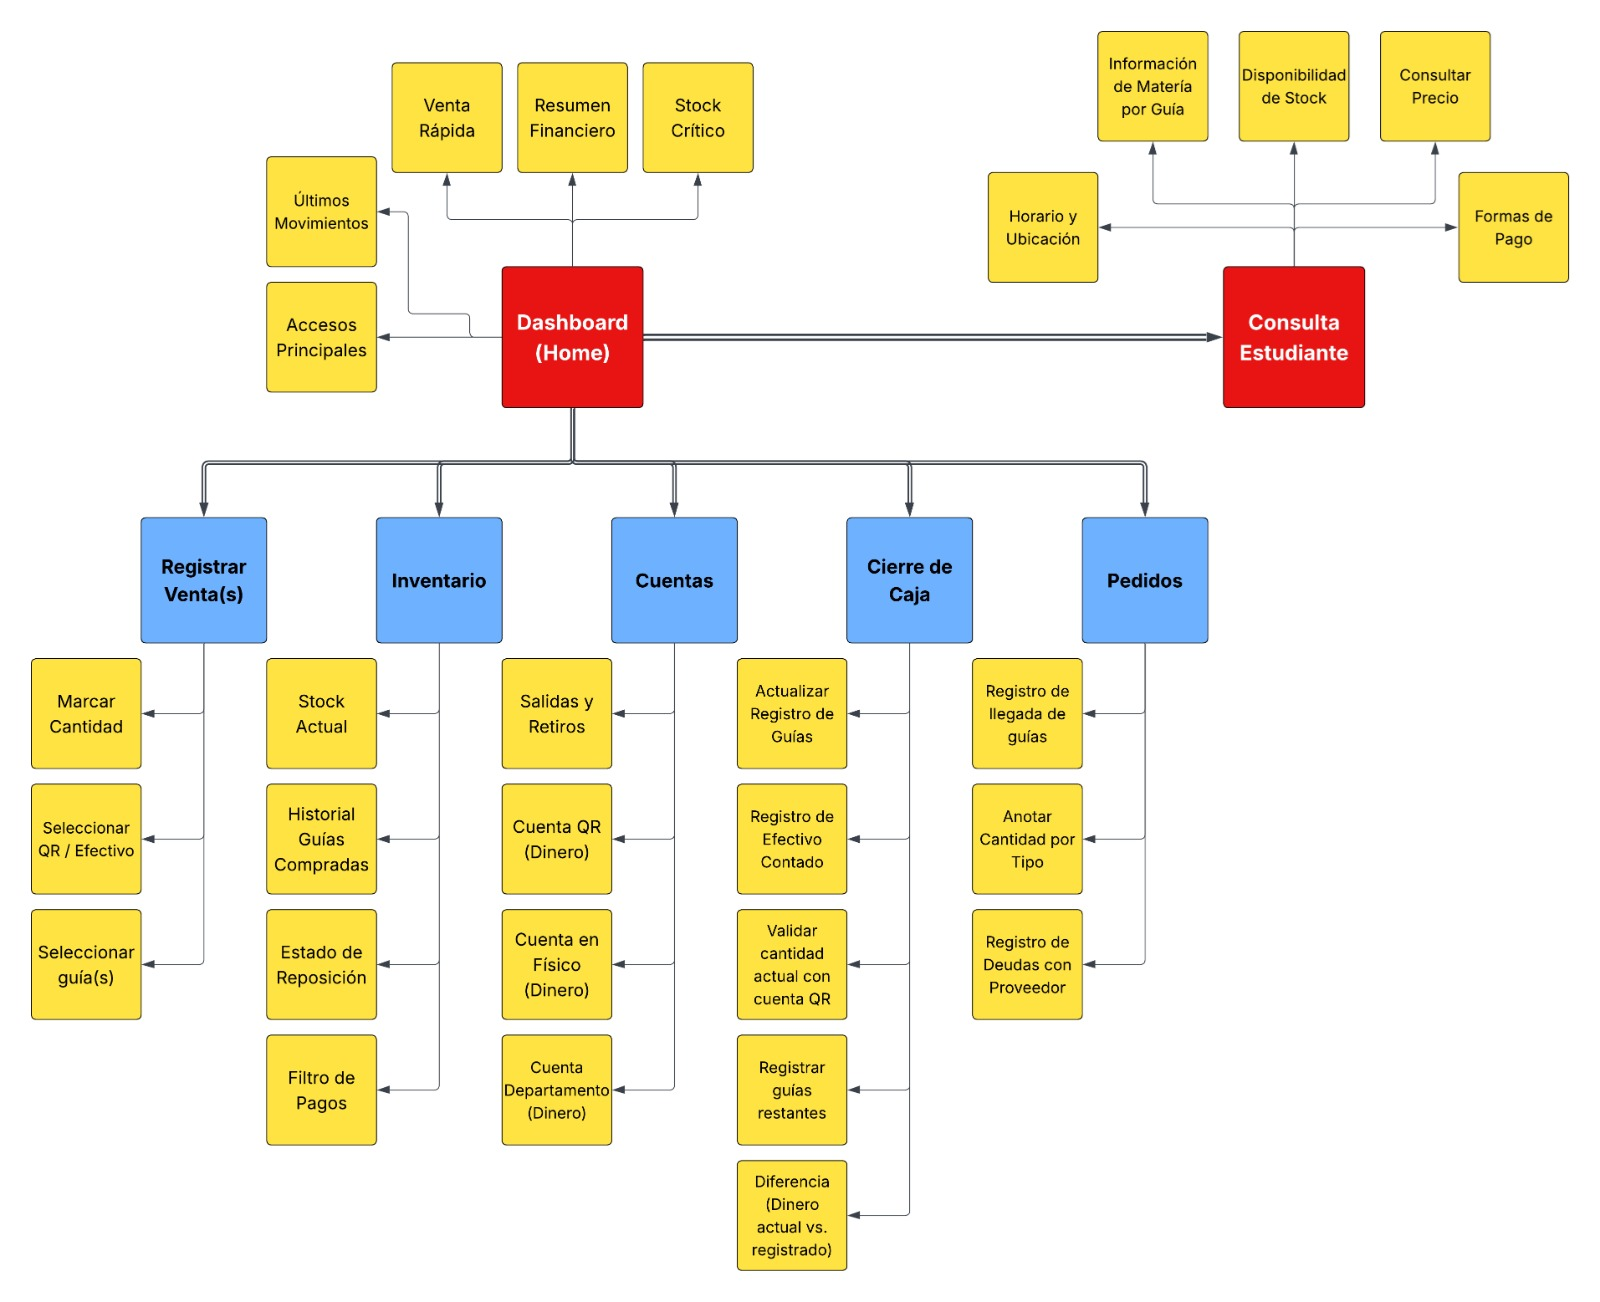
\includegraphics[width=0.9\textwidth,height=0.52\textheight,keepaspectratio]{sitemap.png}
    \caption{Sitemap del prototipo: navegación principal entre Dashboard, ventas, inventario, cuentas, pedidos y consulta de estudiante.}
\end{figure}

La figura resume la estructura de navegación del prototipo y muestra cómo el Dashboard actúa como centro de entrada para tareas administrativas, mientras que la consulta de estudiante permanece accesible como módulo informativo para ambos perfiles.

Esta estructura responde a la necesidad de reducir cambios innecesarios de pantalla. Las tareas más frecuentes se ubican cerca del Dashboard y las funciones compartidas o de consulta quedan separadas para evitar confusiones.

\section{Flujos de navegación}

\subsection{Flujo 1: registro de venta presencial}

Este flujo representa la tarea más frecuente del encargado. El objetivo es que una venta pueda registrarse en pocos pasos y que el sistema actualice el inventario automáticamente.

\begin{enumerate}
    \item El estudiante solicita una guía en el Centro de Estudiantes.
    \item El encargado revisa el stock disponible desde el Dashboard o desde Registrar venta.
    \item El encargado selecciona la guía correspondiente.
    \item Se define la cantidad, normalmente una unidad.
    \item Se selecciona el método de pago: efectivo o QR.
    \item Se registra la venta.
    \item El sistema descuenta el stock y agrega el movimiento al historial.
\end{enumerate}

\subsection{Flujo 2: cierre de caja}

El cierre de caja se identificó como una tarea con mayor carga cognitiva. Por ello, el flujo se plantea como una secuencia guiada.

\begin{enumerate}
    \item El encargado ingresa a Cierre de caja.
    \item Cuenta las guías sobrantes por tipo.
    \item Cuenta el dinero físico disponible.
    \item Revisa el monto reportado por pagos QR.
    \item El sistema compara los valores contados con los valores esperados.
    \item Si todo cuadra, se guarda el cierre.
    \item Si existe diferencia, se registra pérdida o ganancia antes de guardar.
\end{enumerate}

\subsection{Flujo 3: llegada de guías}

Este flujo permite actualizar inventario y deuda con proveedor cuando llega un nuevo pedido.

\begin{enumerate}
    \item Llega un pedido de guías desde la fotocopiadora.
    \item El encargado registra fecha, tipo de guía, cantidad y precio.
    \item Se indica si el pedido fue pagado o queda pendiente.
    \item El sistema actualiza el inventario.
    \item Si queda deuda, se refleja en el resumen administrativo.
\end{enumerate}

\subsection{Flujo 4: consulta del estudiante}

Este flujo responde a la necesidad detectada en los compradores, quienes quieren saber si la guía está disponible antes de acercarse al Centro. También puede ser usado por el encargado cuando necesita verificar información rápida para orientar una consulta.

\begin{enumerate}
    \item El estudiante abre la vista de consulta.
    \item Revisa qué guía corresponde a su materia o carrera.
    \item Verifica stock y precio.
    \item Revisa horario, ubicación y formas de pago.
    \item Si existe disponibilidad, acude al Centro de Estudiantes para comprar presencialmente.
\end{enumerate}

\section{Wireframes de baja fidelidad}

El prototipo inicial fue construido como una aplicación navegable en React, pero su objetivo dentro de esta etapa es representar un mockup de baja fidelidad. Por esa razón, se priorizó la organización de pantallas, jerarquía de información, ubicación de acciones y estructura de navegación, antes que el acabado visual final.

\begin{figure}[H]
    \centering
    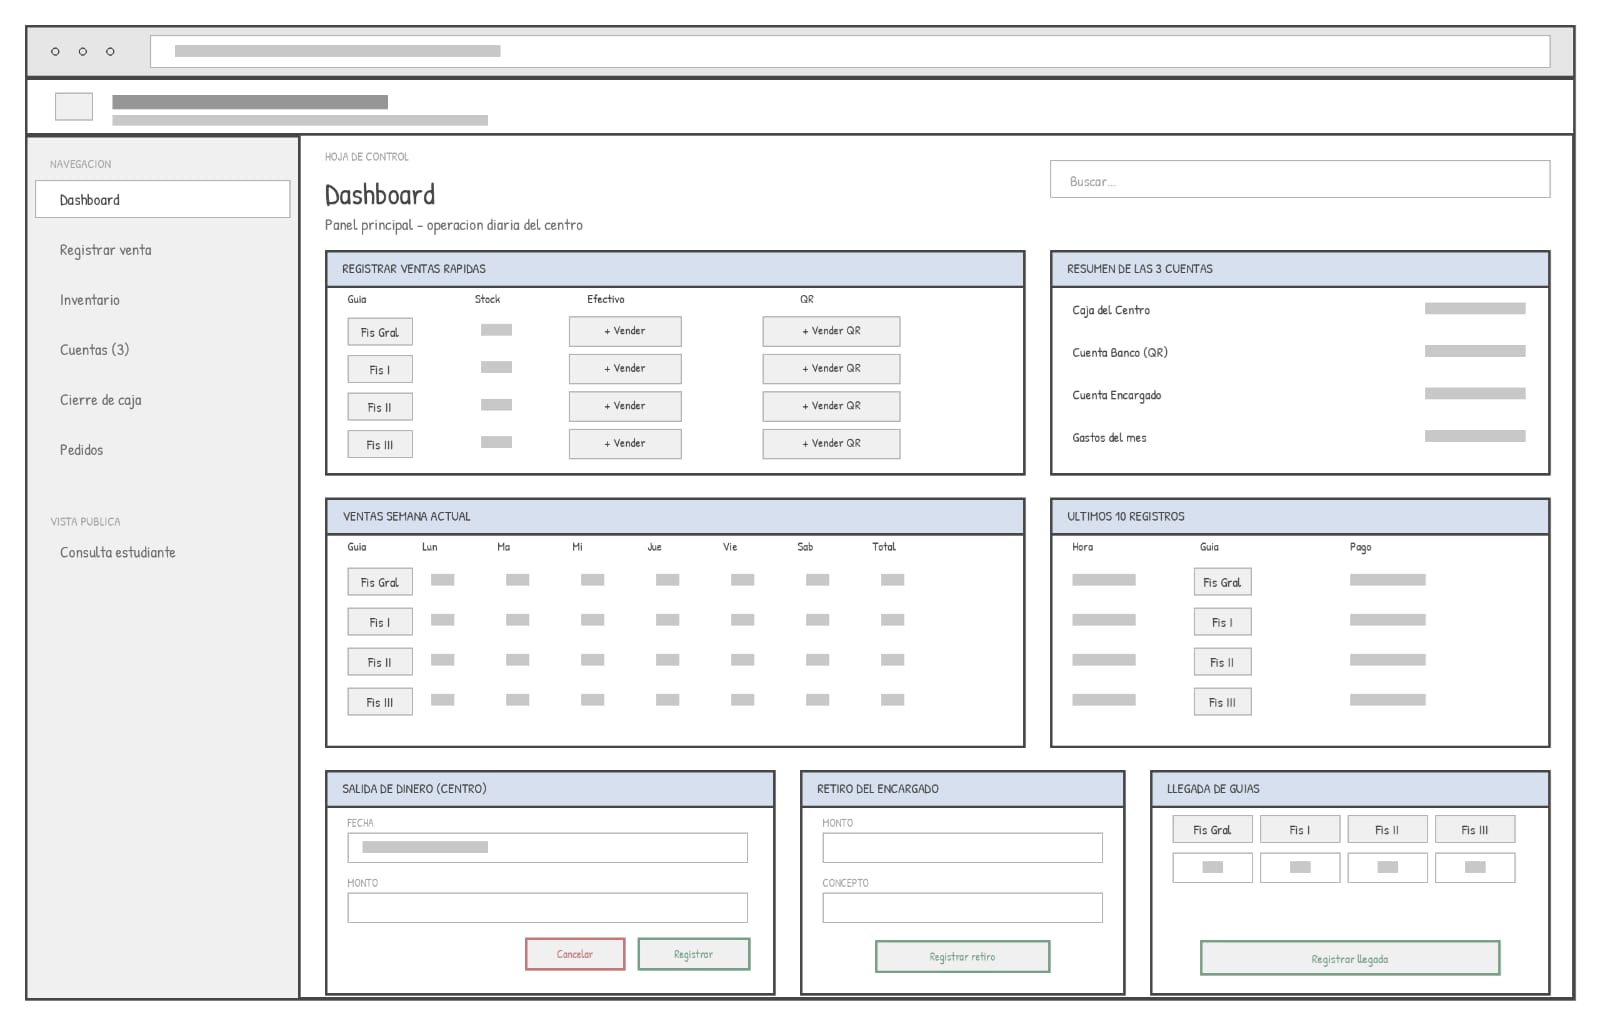
\includegraphics[width=0.95\textwidth,height=0.58\textheight,keepaspectratio]{wireframe_dashboard.png}
    \caption{Wireframe del Dashboard: resumen operativo, ventas rápidas, cuentas e historial.}
\end{figure}

\begin{figure}[H]
    \centering
    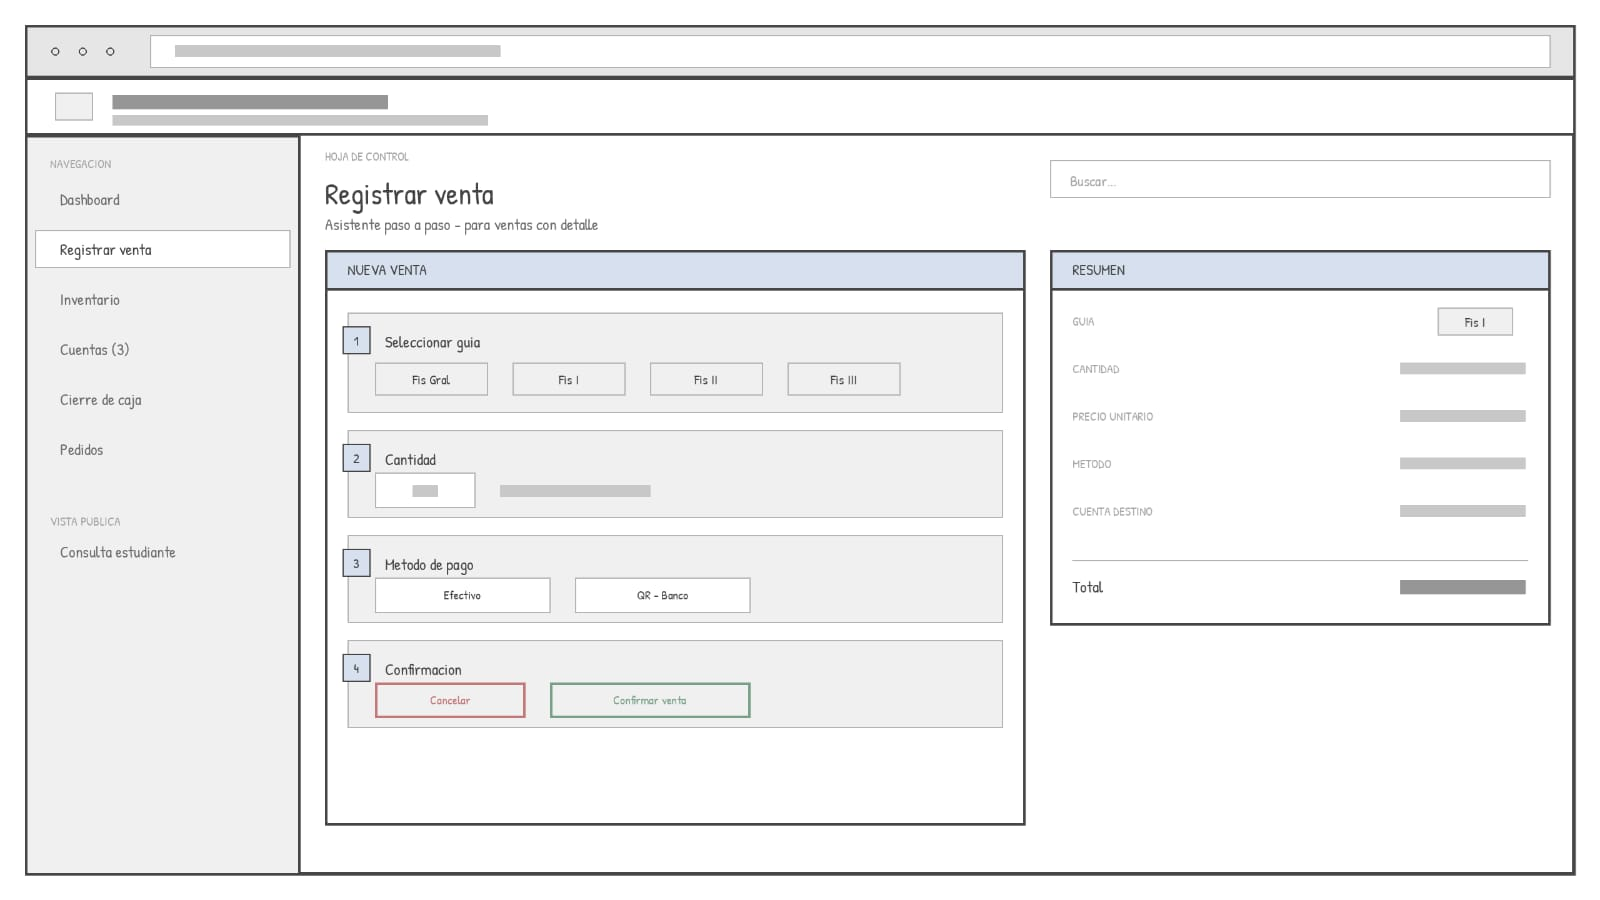
\includegraphics[width=0.95\textwidth,height=0.58\textheight,keepaspectratio]{wireframe_ventas.png}
    \caption{Wireframe de registro de venta: selección de guía, cantidad y método de pago.}
\end{figure}

\begin{figure}[H]
    \centering
    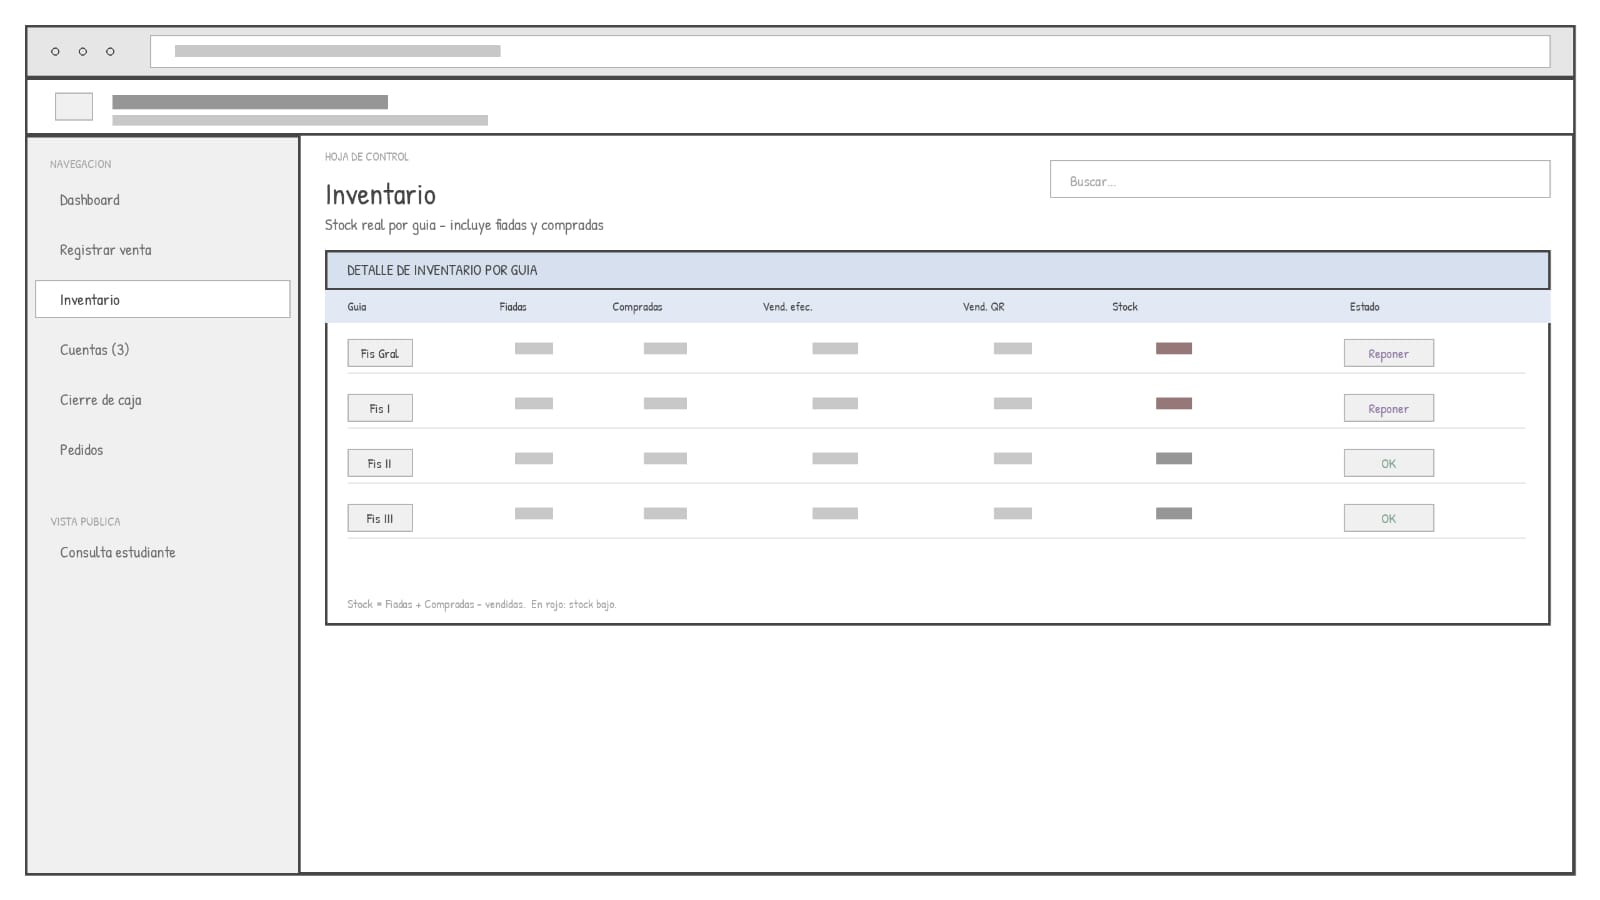
\includegraphics[width=0.95\textwidth,height=0.58\textheight,keepaspectratio]{wireframe_inventario.png}
    \caption{Wireframe de inventario: guías fiadas, compradas, vendidas, stock restante y estado.}
\end{figure}

\begin{figure}[H]
    \centering
    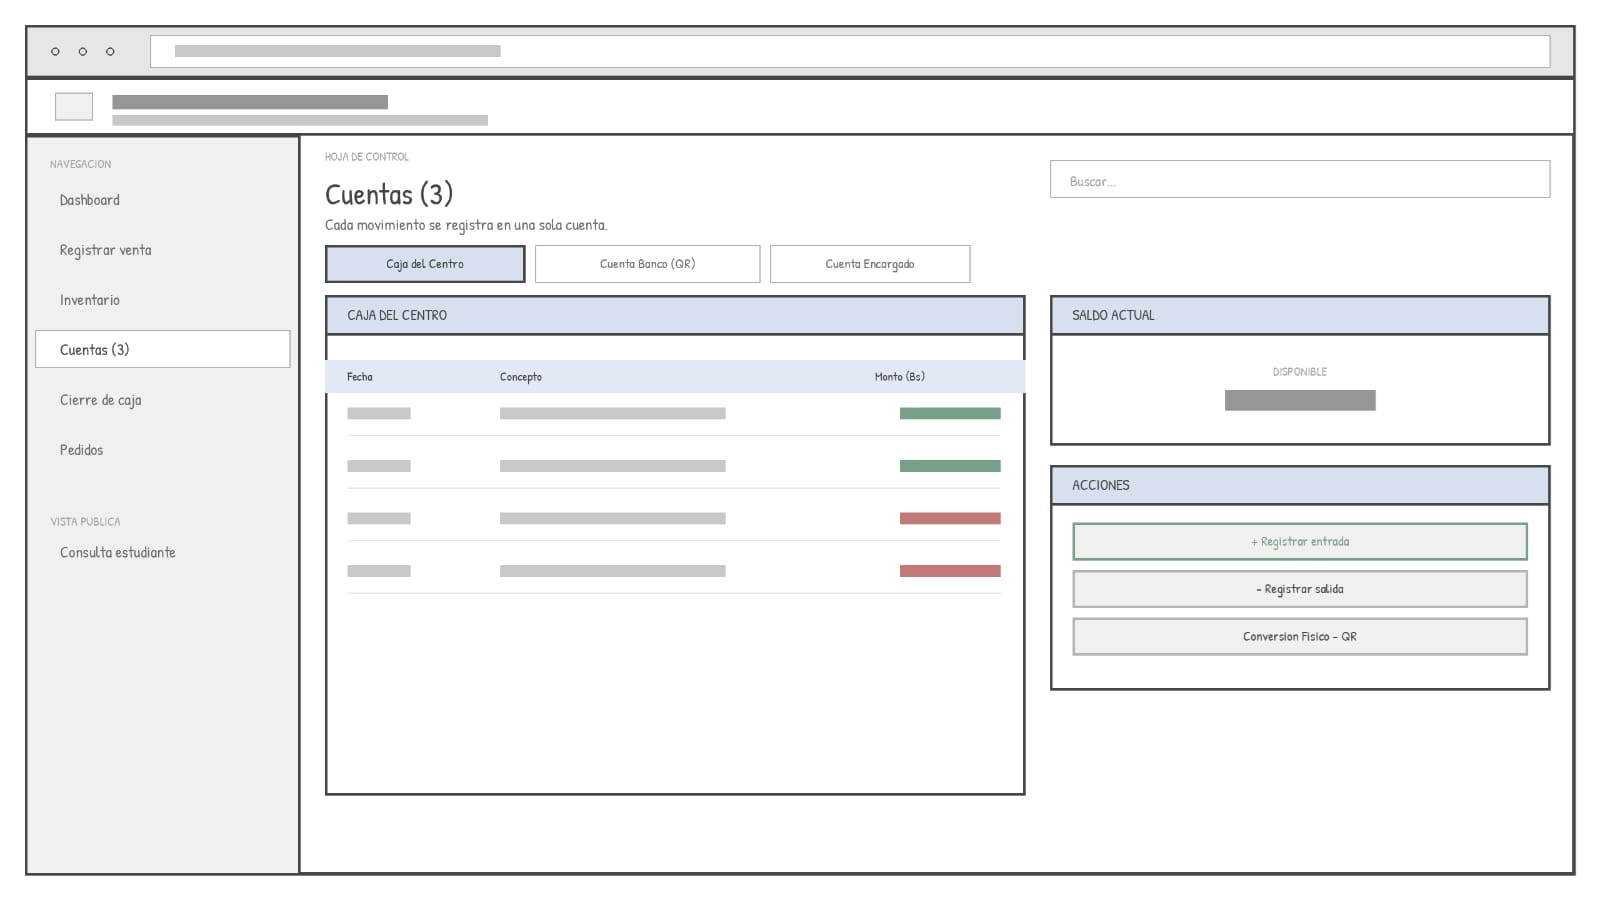
\includegraphics[width=0.95\textwidth,height=0.58\textheight,keepaspectratio]{wireframe_cuentas.png}
    \caption{Wireframe de cuentas: separación entre caja física, cuenta QR y cuenta del encargado.}
\end{figure}

\begin{figure}[H]
    \centering
    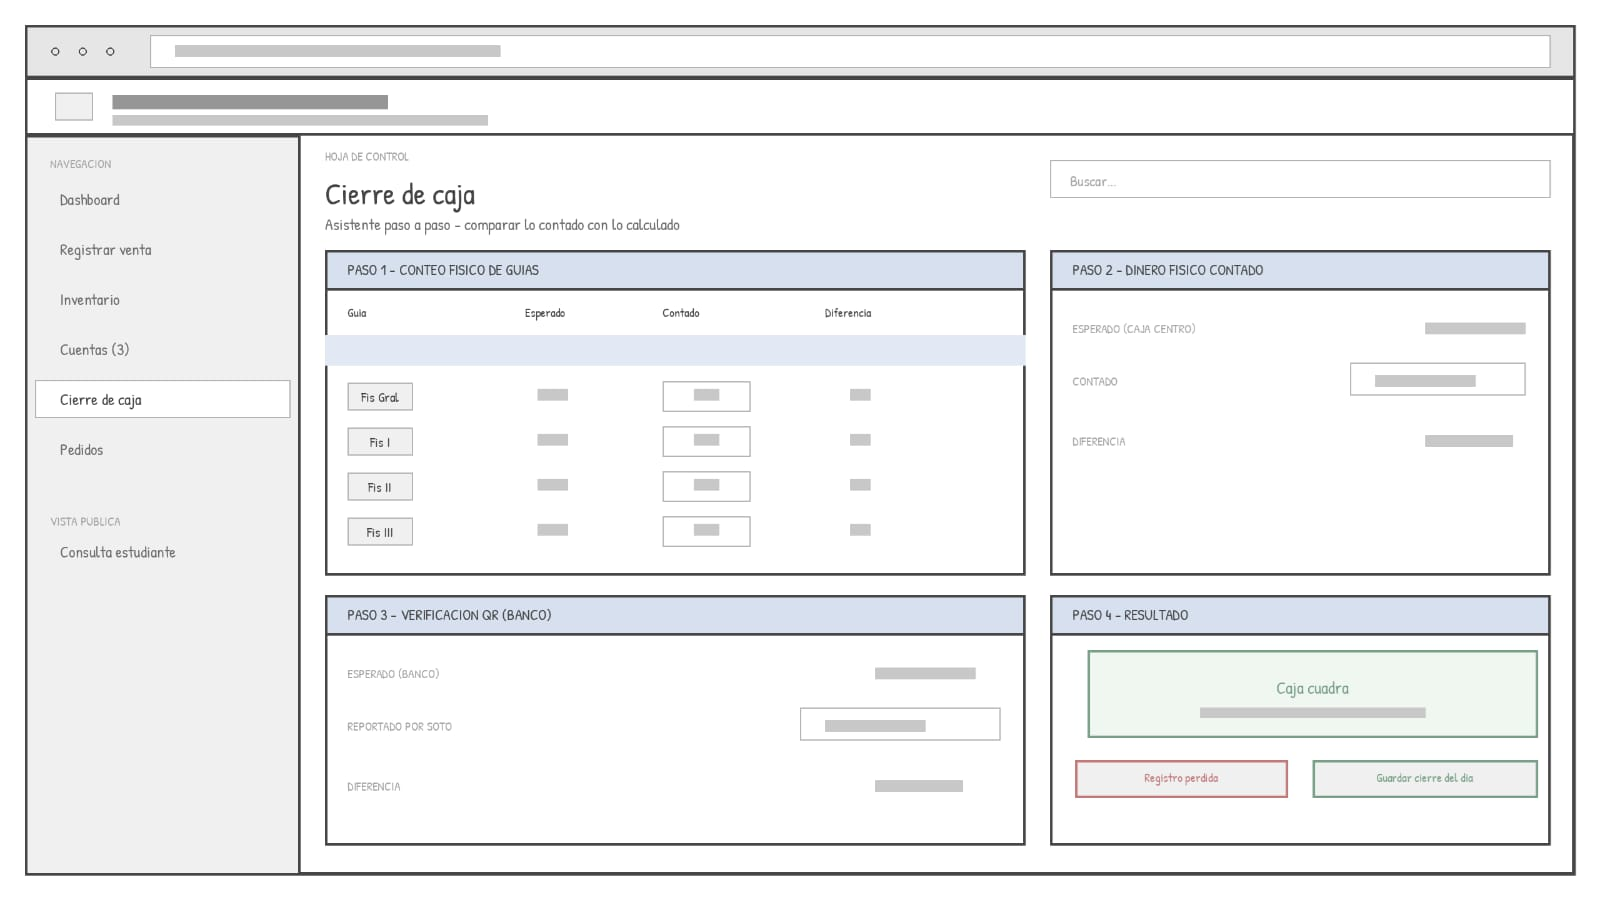
\includegraphics[width=0.95\textwidth,height=0.58\textheight,keepaspectratio]{wireframe_cierre_caja.png}
    \caption{Wireframe de cierre de caja: verificación de guías, dinero físico y pagos QR.}
\end{figure}

\begin{figure}[H]
    \centering
    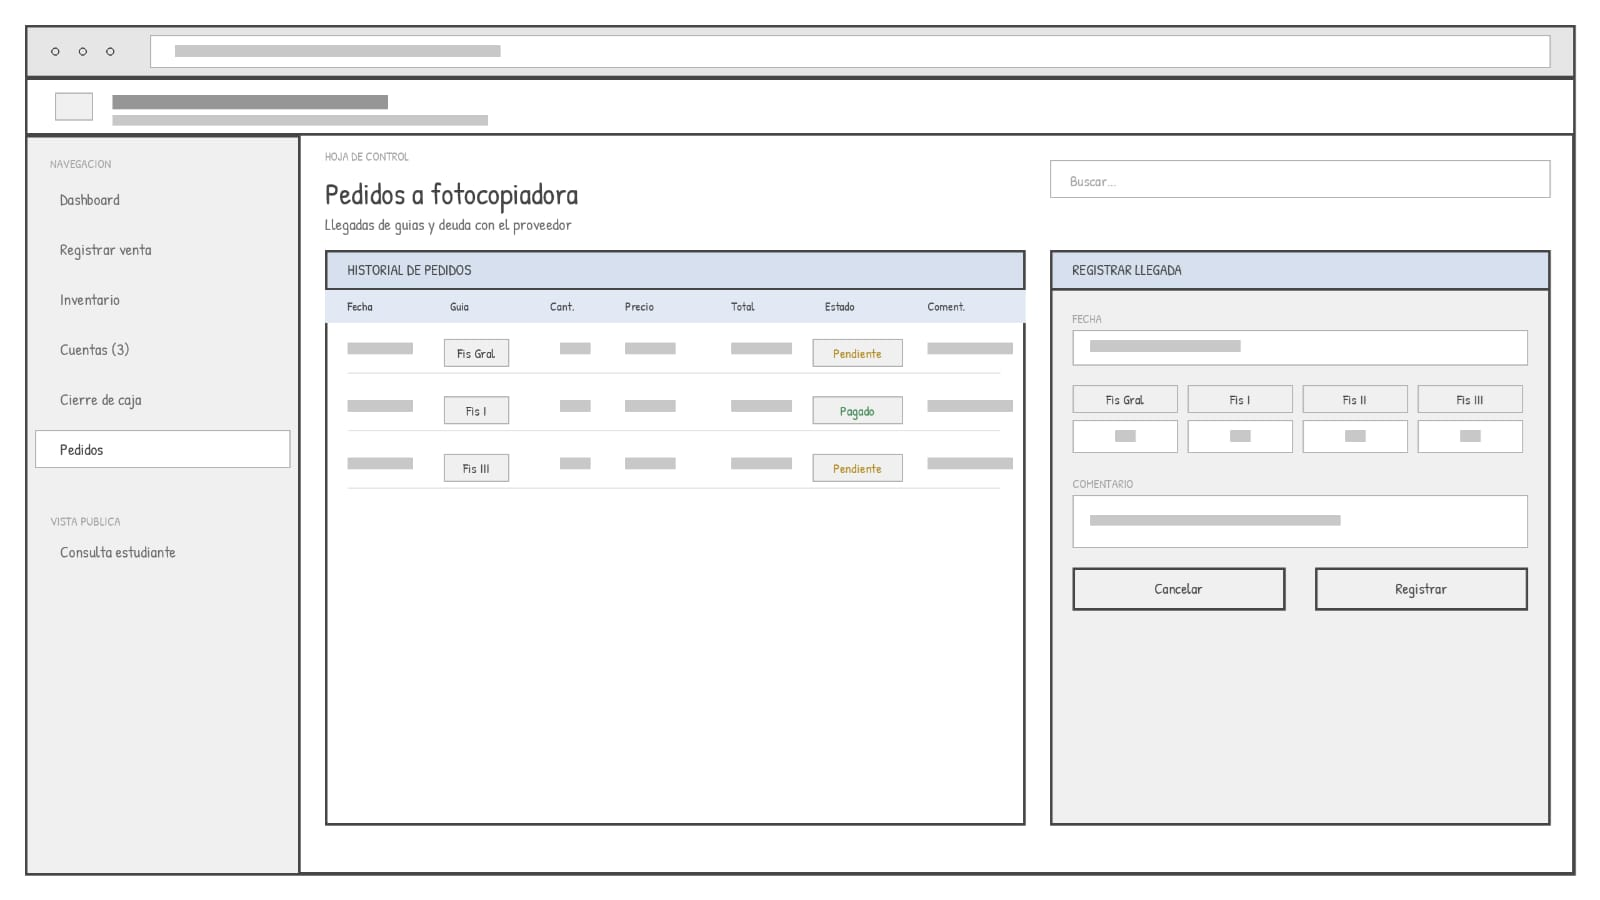
\includegraphics[width=0.95\textwidth,height=0.58\textheight,keepaspectratio]{wireframe_pedidos.png}
    \caption{Wireframe de pedidos: llegadas de guías, costos, estado de pago y deuda.}
\end{figure}

\begin{figure}[H]
    \centering
    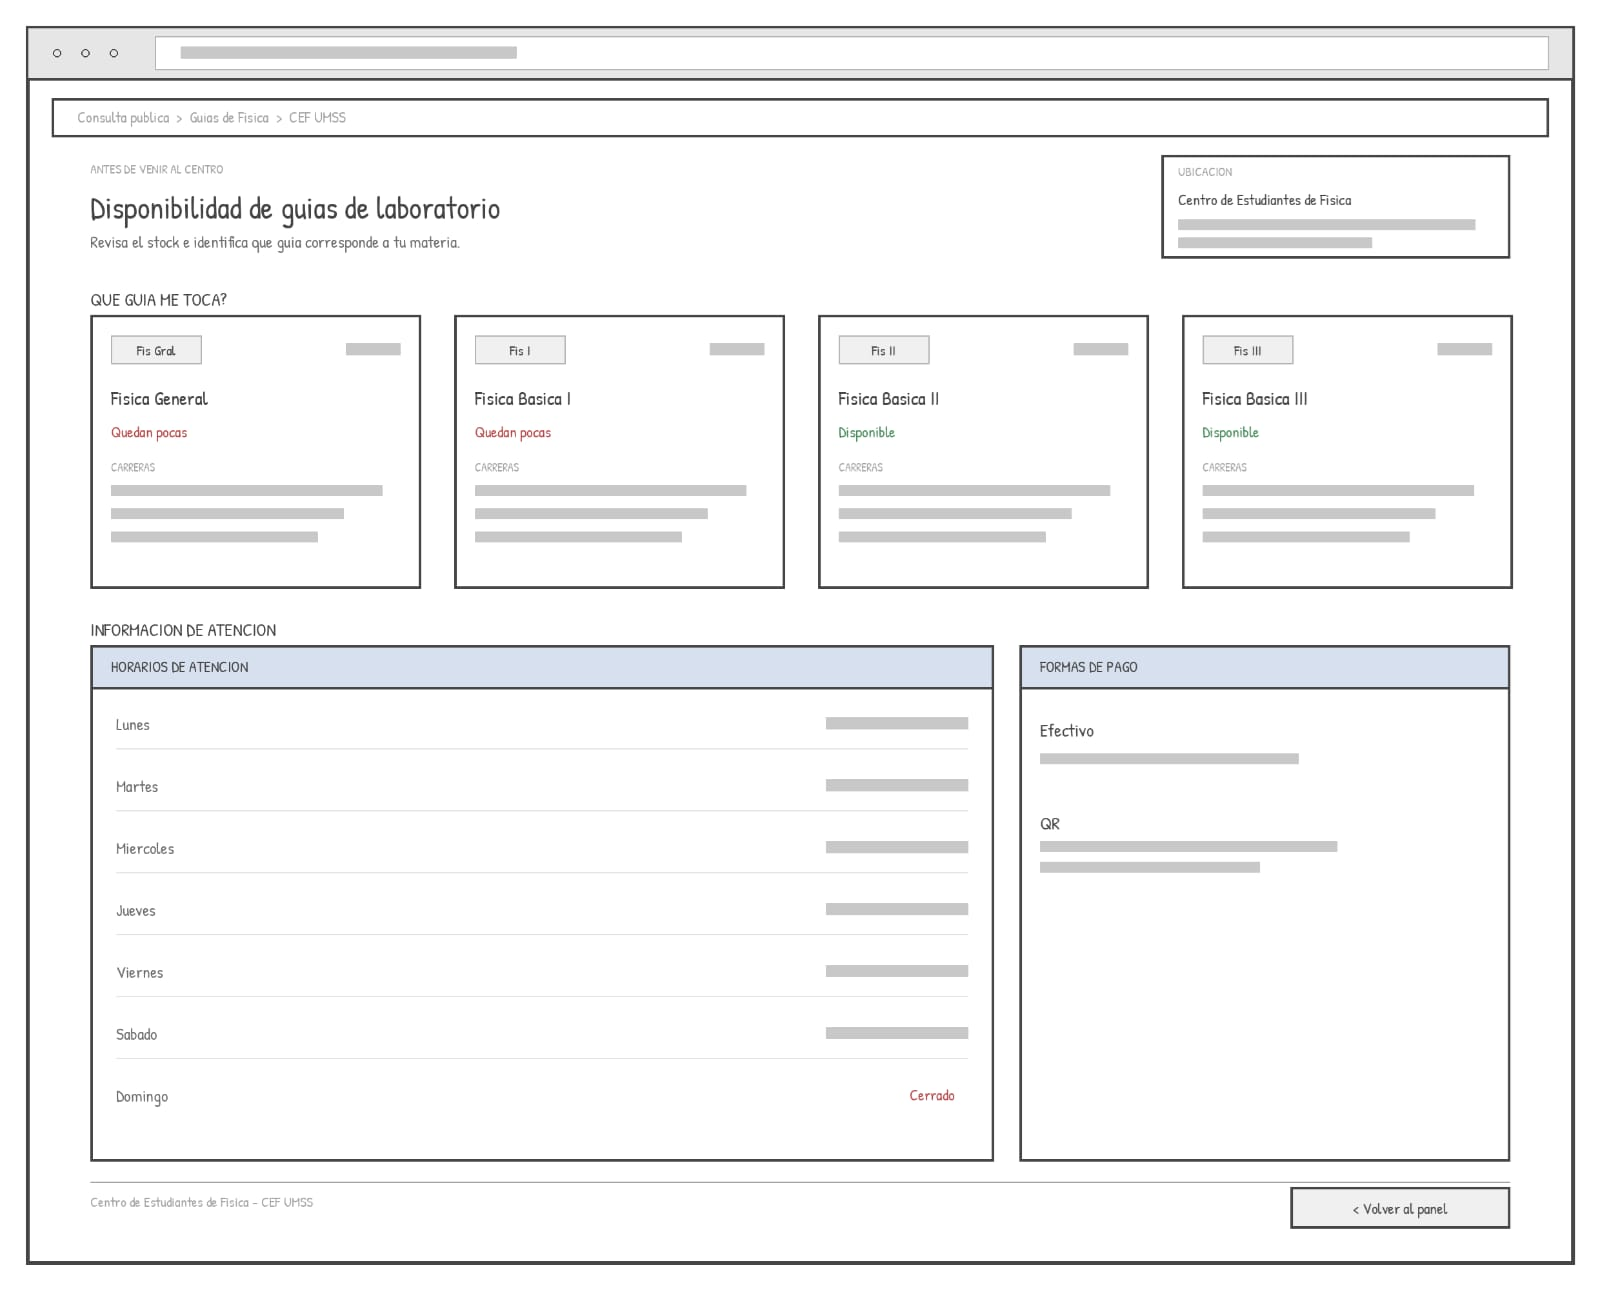
\includegraphics[width=0.95\textwidth,height=0.58\textheight,keepaspectratio]{wireframe_vista_estudiante.png}
    \caption{Wireframe de consulta para estudiantes: disponibilidad, precio, materia y datos de atención.}
\end{figure}

\FloatBarrier

\section{Decisiones de diseño}

\subsection{Navegación lateral}

Se eligió una navegación lateral porque el usuario principal necesita cambiar entre funciones administrativas sin perder el contexto. Esta estructura permite mantener visibles las secciones principales: Dashboard, Registrar venta, Inventario, Cuentas, Cierre de caja, Pedidos y Consulta estudiante.

\subsection{Dashboard como centro de operaciones}

El Dashboard concentra acciones frecuentes y datos de control. Esta decisión evita que el usuario tenga que abrir varias pantallas para realizar tareas simples, como registrar una venta rápida, revisar stock o consultar los últimos movimientos.

\subsection{Separación de cuentas}

La investigación mostró que no todo el dinero se maneja igual. Por ello, el prototipo diferencia caja física, cuenta QR y cuenta del encargado. Esta separación ayuda a comprender de dónde proviene cada monto y facilita la rendición.

\subsection{Vista pública para estudiantes}

Aunque los estudiantes no son usuarios administrativos, se incluyó una vista de consulta porque en la investigación se detectó incertidumbre sobre stock y correspondencia entre guía y materia. Esta pantalla reduce dudas antes de la compra presencial.

\section{Justificación basada en IHC}

\subsection{Usabilidad}

El prototipo busca facilitar las tareas más frecuentes del encargado. Registrar una venta requiere pocos pasos y las acciones principales se presentan en botones visibles. El inventario usa tablas porque los encargados ya están familiarizados con estructuras similares a planillas. El cierre de caja se presenta como una pantalla de verificación para disminuir errores en una tarea sensible.

También se consideró la facilidad de aprendizaje. La navegación usa nombres directos y cercanos al lenguaje del usuario: Registrar venta, Inventario, Cuentas, Cierre de caja y Pedidos. Esto evita términos técnicos innecesarios y permite que un nuevo encargado entienda rápidamente dónde realizar cada acción.

\subsection{Leyes de la Gestalt}

La ley de proximidad se aplica agrupando elementos relacionados dentro de paneles: ventas rápidas, resumen de cuentas, últimos registros, pedidos o cierre. Esta agrupación permite que el usuario interprete cada bloque como una unidad funcional.

La ley de similitud se aplica mediante botones, tablas y etiquetas visuales con estilos consistentes. Las guías se identifican con badges similares, variando solo el color y el texto según el tipo de guía.

La ley de continuidad se refleja en los flujos de uso. Las pantallas siguen una lectura de arriba hacia abajo y de izquierda a derecha, lo que favorece una secuencia natural de trabajo. En el cierre de caja, por ejemplo, primero se revisan las guías, luego el dinero y finalmente las diferencias.

La relación figura-fondo se usa para separar el contenido de trabajo del fondo general. Los paneles claros sobre un fondo suave ayudan a distinguir las áreas de acción sin sobrecargar la vista.

\subsection{Carga cognitiva}

La propuesta intenta reducir la carga cognitiva del encargado al mostrar cálculos como resumen y no como fórmulas. Las operaciones complejas se dividen en pasos, especialmente en el cierre de caja. Además, las acciones frecuentes están disponibles desde el Dashboard, lo cual disminuye la necesidad de recordar rutas o procedimientos largos.

El uso de colores para las guías funciona como apoyo visual, pero no como única forma de identificación. Cada guía también tiene texto, materia y datos numéricos, evitando depender solamente del color.

\section{Relación con los hallazgos de usuarios}

Las decisiones de arquitectura y diseño responden a los problemas detectados en la investigación. Los encargados necesitaban mayor claridad para ventas, stock, dinero y cierre de caja; por eso se definieron pantallas separadas pero conectadas. Los estudiantes compradores necesitaban información previa antes de ir al Centro; por eso se incluyó una vista pública de consulta.

\begin{center}
\begin{tabularx}{\textwidth}{|B{5cm}|Y|}
\hline
Hallazgo de investigación & Decisión aplicada en el prototipo \\
\hline
Los encargados registran ventas y revisan stock con frecuencia. & Se agregó venta rápida y stock visible en el Dashboard. \\
\hline
El cierre de caja puede resultar confuso. & Se diseñó una pantalla de cierre con pasos de verificación y comparación. \\
\hline
Se necesita trazabilidad de movimientos. & Se incluyó historial de últimos registros y secciones de cuentas/movimientos. \\
\hline
Los estudiantes no siempre saben si hay stock. & Se agregó una vista de consulta con disponibilidad y precio. \\
\hline
Existe duda sobre qué guía corresponde a cada materia. & La vista de consulta relaciona guía, materia y carreras asociadas. \\
\hline
\end{tabularx}
\end{center}

\end{document}

